%\flushleft

What did we do to ensure the quality of our final product? 

To ensure the development stayed on track and produced useable and useful code, our User Stories adhered to the INVEST criteria as much as practical, always detailing a specific feature either wanted by the client or seen as necessary by the Team for the inner workings of the program. 
However, we had to deviate from the template to adjust to the peculiarities of the project at hand:
The limited time of roughly 80 manhours total per sprint made it impractical to limit a userstory to "one third of a sprint"; Most often, a single sprint consisted of between two and three user stories, each of which spanned at least half a sprint to implement by between one and four people. 
\paragraph{INVEST} 
The criteria and how closely we managed to follow them:
\begin{table}[h!]
  \caption{INVEST}
  \label{INVEST}
  \centering
  \begin{tabular}{|p{3cm} | p{10cm}|}
	\hline  	 
  	 Criteria & Comments \\ 
  	 \hline
  	 \hline
  	Independent & User Stories should be independent of each other if at all possible. Due to the nature of the project, some stories could not be fully independent: for Example, '\# 24 Display Analysis Data' would depend on actual data being present, as generated by code created in User Story \# 23. In general, all our UI-related stories require the results of work on the backend.  \\ 
  	\hline
  	 Negotiable & User Stories should describe what should be done, but not how. The details are to be decided upon in the tasks. We managed to adhere to this over all User Stories.  \\ 
  	\hline
  	Valuable & A User Story needs to specify a clear benefit to the customer. All our User Stories have a benefit to the customer, but in some cases, amongst other things our backend, the benefit may not be easily recognizable by the customer. Thus, some of our User Stories were not written from a customers perspective. \\ 
  	\hline
  	Estimable & A Story's size should always be estimable, whether by elaborate method or an educated guess. As we did have no experience in working as a team, we categorized stories roughly into three sizes: L, M, S.  Within that framework, our size estimates were relatively accurate.   \\ 
  	\hline
  	  \end{tabular}
\end{table}
\begin{table}[h!]
  \caption{INVEST: cont}
  \centering
  \begin{tabular}{|p{3cm} | p{10cm}|}
	\hline  	 
  	 Criteria & Comments \\ 
  	 \hline
  	 \hline
  	Small & User Stories should be no larger than one third of a sprint. Due to the limited amount of work time in a sprint, less than 20 hours per team member, we frequently did not manage to adhere to this principle. Early sprints only had two user stories each.  \\ 
  	\hline
  	Testable & To see if a User Story is complete, it desired result needs to be confirm-able by acceptance tests. Our stories generally have success criteria that can be tested against, though in the case of the GUI this was largely done by manual testing, as the team judged writing GUI tests to be too time-consuming to consider. \\ 
  	\hline
  \end{tabular}
\end{table}

\paragraph{Example user story card} \
The Story below has an estimated size, a defined and testable goal, and is important to the project. How exactly it is to be done is not part of the user story, instead being detailed in the respective tasks, or decided by the assigned team member at the time of implementation. 
\begin{table}[h]
  \caption{User Story 7: Testrun Table, Front}
  \label{Story 7 Example}
  \centering
  \begin{tabular}{|p{9cm} p{2cm}|}
	\hline  	
  	Testrun Table & Nr. 7.001  \\ 
  	\hline
  	As a user, &    \\ 
  	I want to display a table containing all the classes of one specific testrun and their failure percentage so that I can get a quick overview of the most problematic classes. &    \\ 
  	Size: M & Sprint: 2 \\ 
  	\hline
  \end{tabular}
\end{table}
\begin{table}[!h]
  \caption{User Story 7: Testrun Table, Back}
  \label{Story 7 Example}  \centering
  \begin{tabular}{|p{10cm} p{1cm}|}
    \hline
  	  &    \\ 
  	The story is done when &    \\ 
  	 - the classes are sorted in decending order of failure percentage &    \\ 
  	 - the classes with the highest failure percentage are highlighted &   \\ 
  	  &     \\ 
  	\hline
  \end{tabular}
\end{table}

\paragraph{Tasks} 
When it came to Tasks, our team only gradually realized the practical importance of the \textbf{ SMART}-criteria; over the course of the project our organization improved.


\begin{table}[h!]
  \caption{SMART}
  \label{SMART}
  \centering
  \begin{tabular}{|p{3cm} | p{5cm}| p{5cm}|}
	\hline  	 
  	 Criteria & Meaning & did we follow it? \\ 
  	 \hline
  	 \hline
  	\hfill \break SPECIFIC & 
  	The task describes an increment of work in sufficient detail in unambiguous words consistent with terminology in the rest of the Project & 
  	 Early on, not all out tasks fulfilled this criteria because we hadn't sufficiently defined our terminology. Some tasks encompassed to much work to possibly  be concise. This improved significantly over the course of the project.\\ 
  	\hline
  	\hfill \break MEASURABLE &
  	 The Task Goal is measurable so the team can test against it's completion & The goal of the teams tasks was always clear enough to be measurable. \\ 
  	\hline
  	\hfill \break ACHIEVABLE &
  	 The task goal shall be achievable by the assigned team member &
  	 We supported each other whenever a teammember had a problem. In a few cases, tasks were aborted after it was revealed they weren't doable within given constraints (like time).   \\ 
  	\hline
  	\hfill \break RELEVANT &
  	 The task clearly contributes to the containing User Story & 
  	 All our tasks contributed to the goals set by the User Story   \\ 
  	\hline
  	\hfill \break TIME BOXED &
  	 The task is limited to a specific duration before the assigned team member(s) seek help & Most our tasks were limited to a single 4-hour meeting through the length of the containing User Story. Some tasks, mostly relating to Apriori, took significantly longer. 
  	    \\ 
  	\hline
  	  \end{tabular}
\end{table}

When we kicked off the project, we created User Stories for Project Goals that we wanted to tackle in later Sprints, and didn't update them after gathering knowledge; This resulted in tasks like the "Implement Apriori", as already detailed above.
\newpage

\begin{table}
  \label{Example Task 1: 8.1}
  \centering
	\begin{tabular}[!th]{ |p{3.5cm} p{2.7cm}| }
	\hline
	Implement Apriori \hfill \break & \multicolumn{1}{r}{8.1} \\
	 . & \\
	 \hfill \break
	 L & \hfill \break Assigned : Jan \\
	 \hline
	\end{tabular}
\end{table}

The task encompassed pretty much the entire User Story (Size \textbf{L}), didn't describe how, and contained no further info, as we didn't have that info when we created it. Neither the story, not the task were updated after research.

\begin{table}
  \label{Example Task 2: 23.1}
  \centering
	\begin{tabular}[!h]{ |p{3.5cm} p{2.7cm}| }
	\hline
	Get failed classes of one test run & \multicolumn{1}{r}{23.1} \\
	 . & \\
	 \hfill \break \break
	 S & Assigned To: \break Tobias Schwartz, \break Jan Martin \\
	 \hline
	\end{tabular}
\end{table}
Newer tasks often concerned themselves with a more clearly defined goal, becoming smaller and more easily estimated in the process. 

\paragraph{Unit Tests}
To confirm the correct functionality of our code, we employed JUnit tests, testing specified methods in a vacuum and comparing the outputs. 
The original idea was to write tests after completing a class, but the priority for unit tests was generally seen as lower than that of implementing required features. Thus, our test coverage was lower closer we got to the completion of crucial features. 
The team invested a significant portion of time in Sprint 5 to increase Test coverage wherever possible, though we didn't manage to get full coverage. 
Classes primarily concerned with the GUI went mostly untested due to a lack of time and technical knowledge on our part. 

\paragraph{JDoc internal documentation}
Well documented code is easier to read, understand, and work on, and thus improves workflow and program quality. Especially during the middle sprints, our documentation was woefully lacking, reducing our efficiency when returning to previously written code. We tried to remedy this problem Starting in Sprint 4, but didn't manage to fully document all our classes.

\paragraph{Acceptance Tests}
To measure if a User Story has been successfully completed, Acceptance Tests can be used to confirm that the program is running within expectations. 
We mostly employed these tests for our GUI classes, frequently writing code, testing it, then adapting or fixing it based on the result. 
However, we did not document these tasks, as the desired result was often described in the User Story, and the tests were done by the team members tasked with the story. In a longer project, or a larger team, better documentation and potentially testing-tasks would certainly be required to prevent confusion.

\newpage
\textbf{DEPCRECATED}
When it came to Tasks, our team only gradually realized the practical importance of the "Specific" in the \textbf{ SMART}-criteria; our early User Stories frequently only contained one or two Tasks, like "Implement Apriori". This became an apparent problem when we tried to improve our documentation in Sprint 4, and we found progress was very hard to track when two people worked on a single task for the majority of a sprint. 
Following this revelation, tasks were created based on what part of the code they concerned themselves with, like refactoring a single class, or a single function, for example the implementation of a distance calculation that spanned multiple classes but could still be linked to a single userstory and completed by a single teammember or a team of two. 
This also made the effort required for a single task more easily measurable and allowed us to track our progress in greater detail. A good example of this would be the difference between user stories 8 and 23, both concerning themselves with the implementation of the Apriori algorithm.

To ensure the working condition of our software, we employed extensive tests of internal methods wherever applicable. 
This includes all internal classes excepting the controller and model classes that frequently contain too many links to other classes, making testing them alone impractical. Most of the methods in those classes are indirectly tested through the tests of the classes they call upon. 


\emph{(Approx.~4--7~pages of text.)}

\emph{Describe and justify the different quality assurance techniques that your group has applied alongside the project's conduct, including the INVEST criteria for the user stories, SMART criteria for the tasks derived from user stories, unit tests for your code, and others.  Illustrate your approach to quality assurance by giving relevant examples for each employed technique. Finally, do not forget to evaluate your software's interfaces (including the GUI).}

\newpage

\ \\
\textbf{Activity Diagrams}\\
\ \\
The following activity diagrams were also used as a means of assuring the quality and logical work-flow of our product. They show how a normal user activity works internally and which actions shall and can be taken by the user.\\ 
In figure \ref{AD-SaP} the activity of selecting and parsing a file/multiple files/a folder is displayed with the end-point not being a indication of the program terminating, but instead just an end to this activity. In the next activity diagram in figure \ref{AD-CToOTR}, the previous activity "select and parse files" is nested inside it, due teo space restrictions and because the user is able to, but doesn't have to also execute the task "display class table of one testrun" after parsing. The last figure \ref{AD-DCCoTR} shows the "display class chart over testruns" activity and contains the previous two activities again, because of the same reasons previously mentioned. These diagrams were of great help during the development process, as they gave a clear overview over the logical sequence of actions and brought some errors in our code to our attention: for example, we previously did not switch our center GUI-window to chart tab, even though this was only logical to do. Due to the diagram \ref{AD-DCCoTR}, we spotted this overlooked error in our code and fixed it. This was also only possible, because the diagram was based, but not restricted to our code and we adapted both bi-directional.\\
\ \\
\begin{figure}[h]
\begin{center}
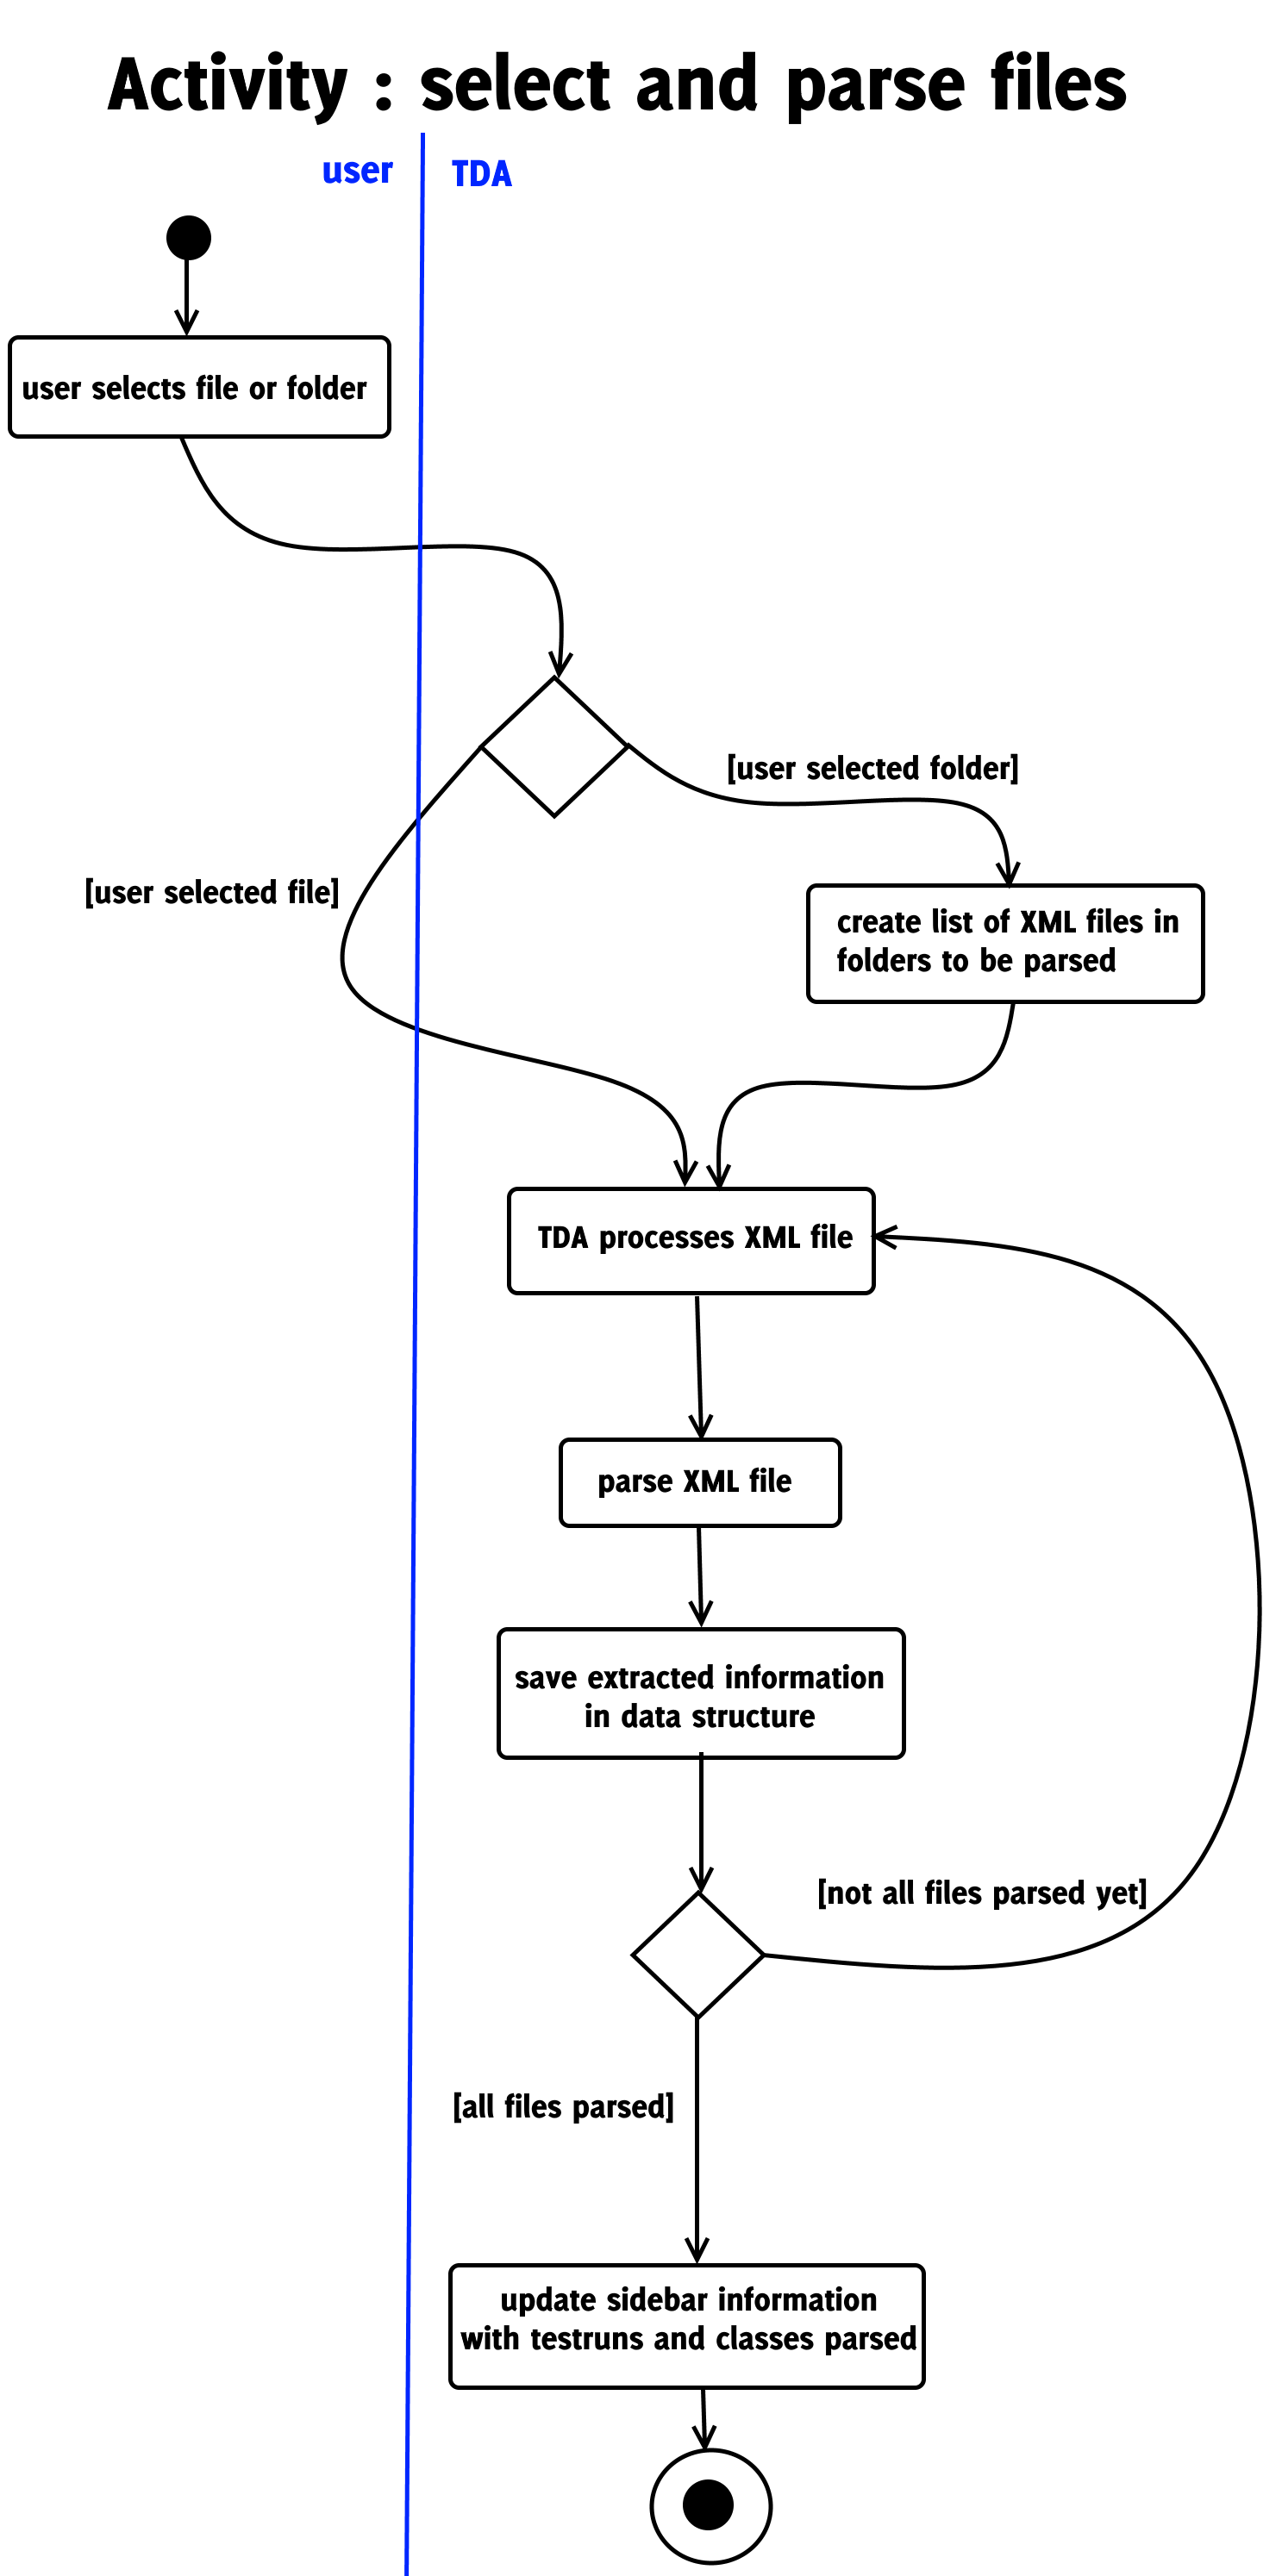
\includegraphics[scale=0.27]{pics/activityDiagramSelectAndParseFiles.png}
\caption{Activity Diagram: select and parse files} 
\label{AD-SaP}
\end{center}
\end{figure}
\ \\
\begin{figure}[h]
\begin{center}
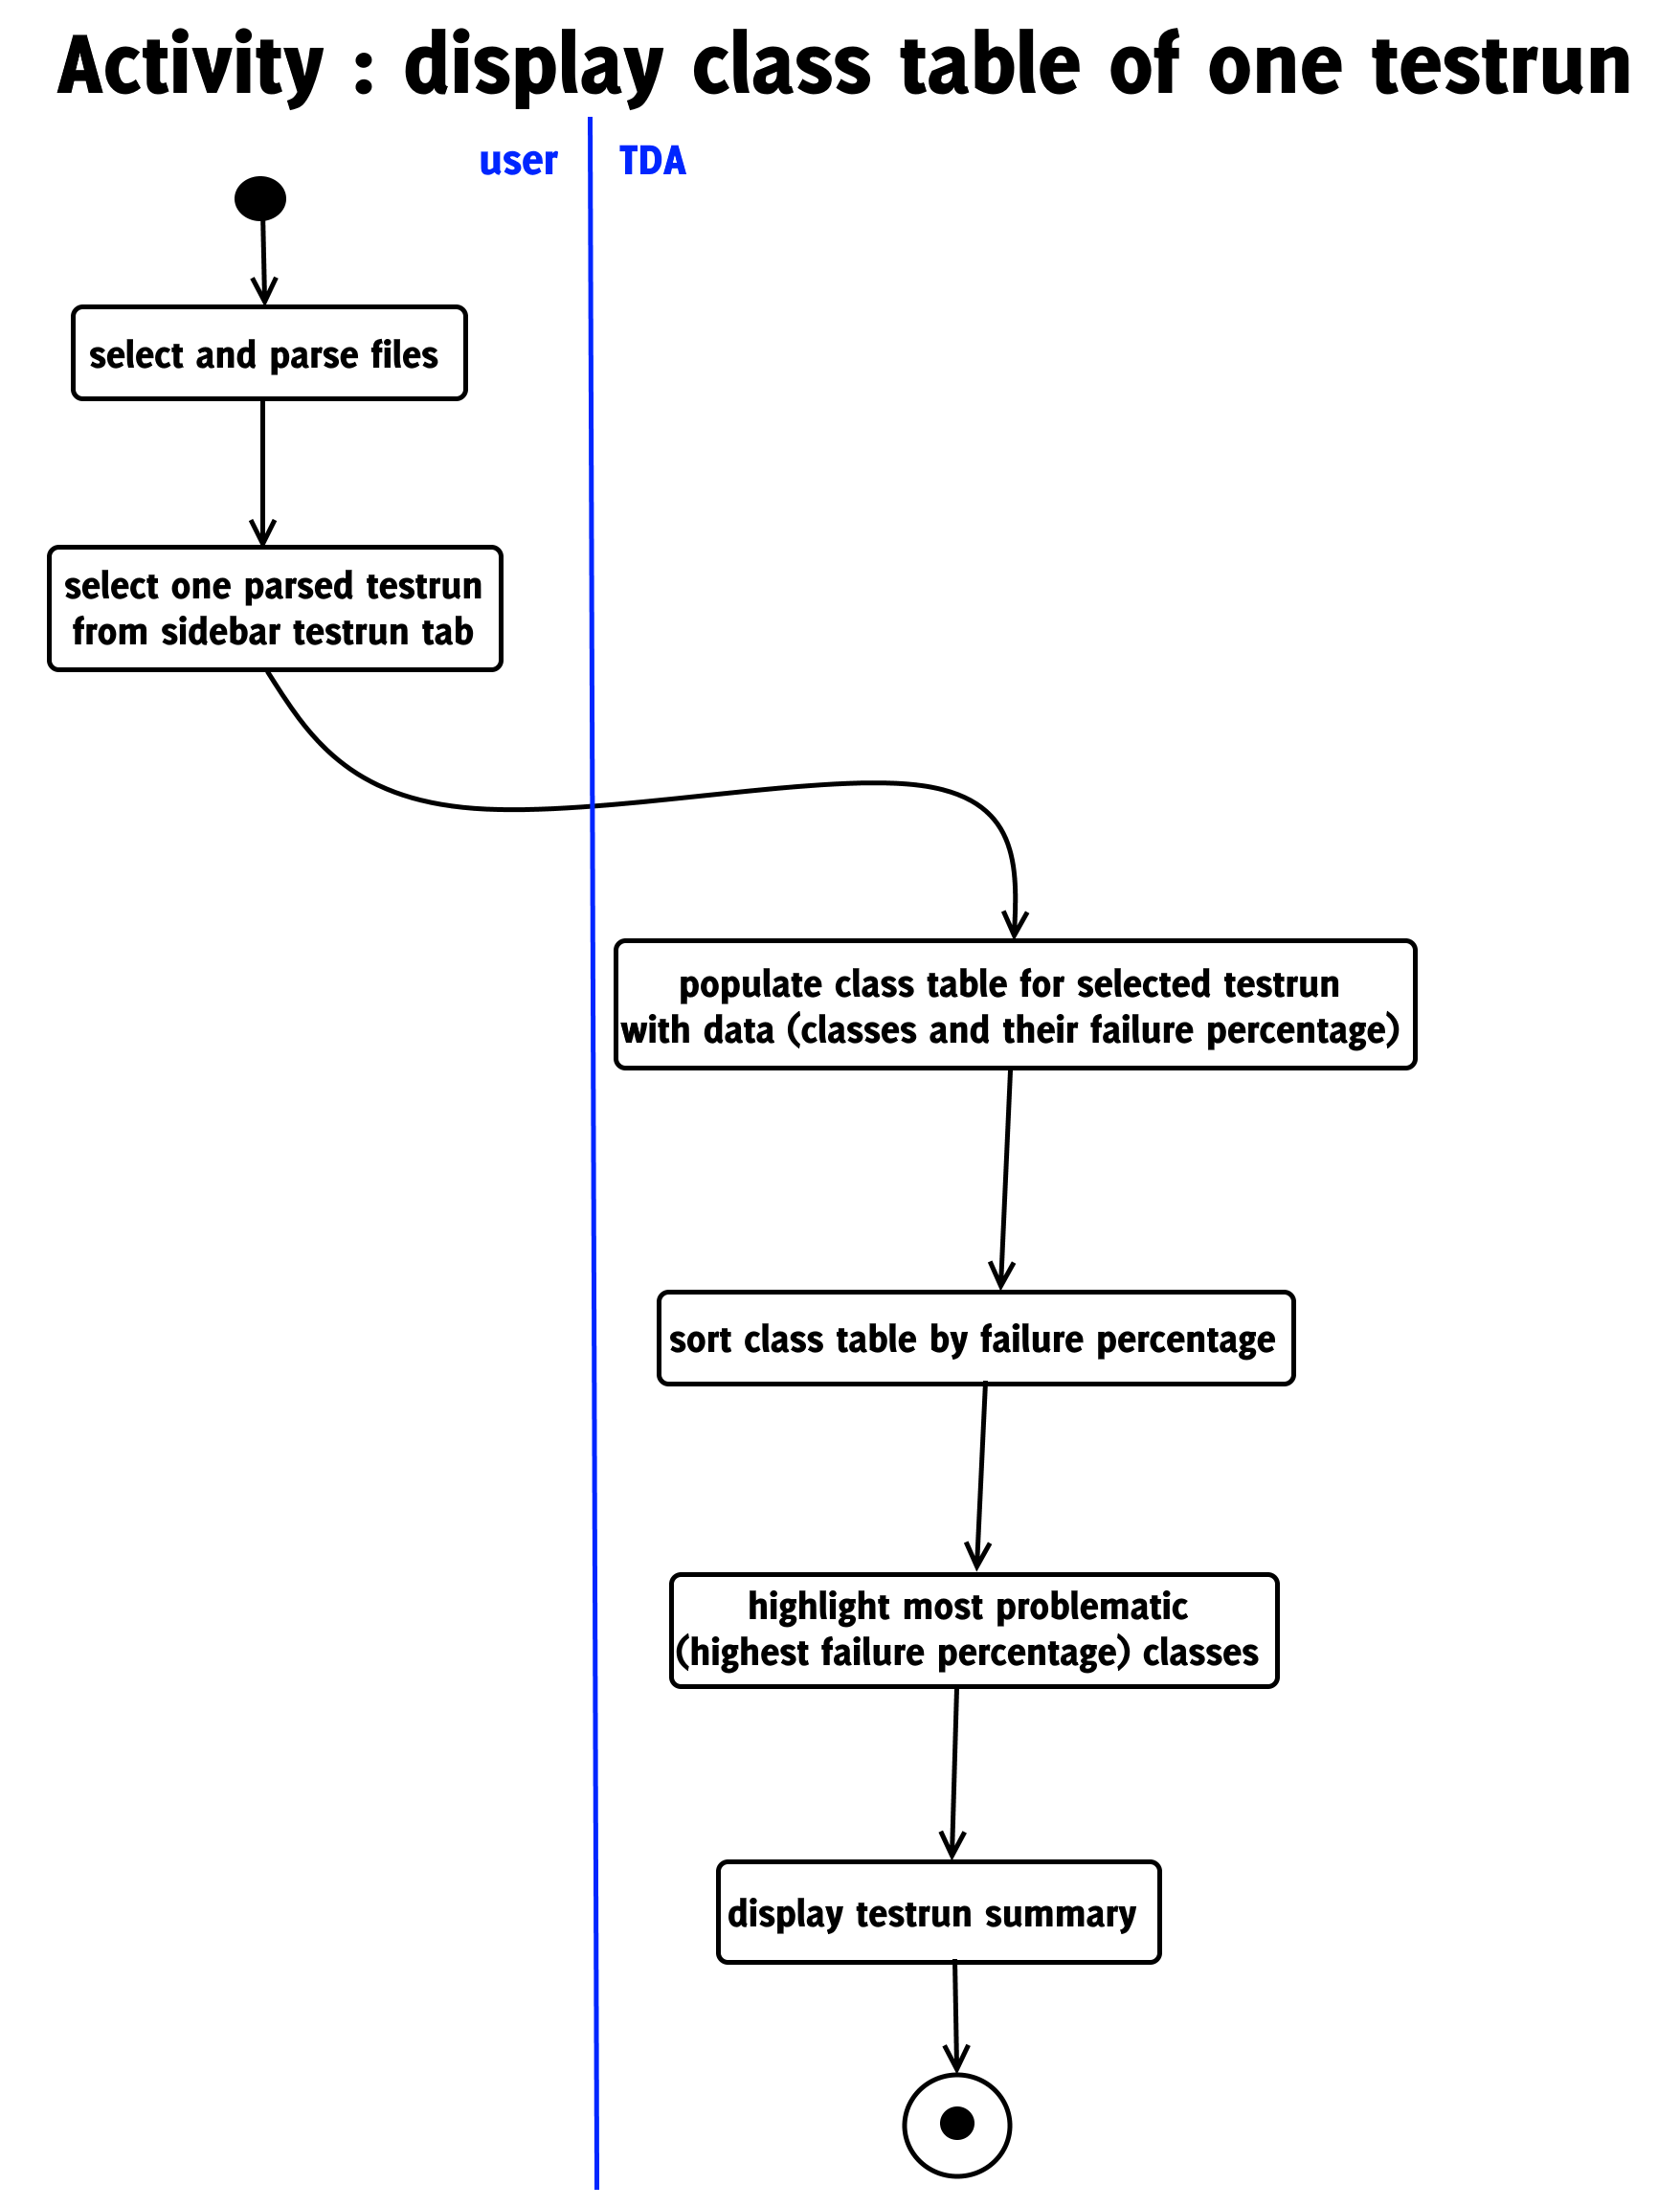
\includegraphics[scale=0.3]{pics/activityDisplayClassTableOfOneTestrun.png}
\caption{Activity Diagram: display class table of one testrun} 
\label{AD-CToOTR}
\end{center}
\end{figure}
\ \\
\begin{figure}[h]
\begin{center}
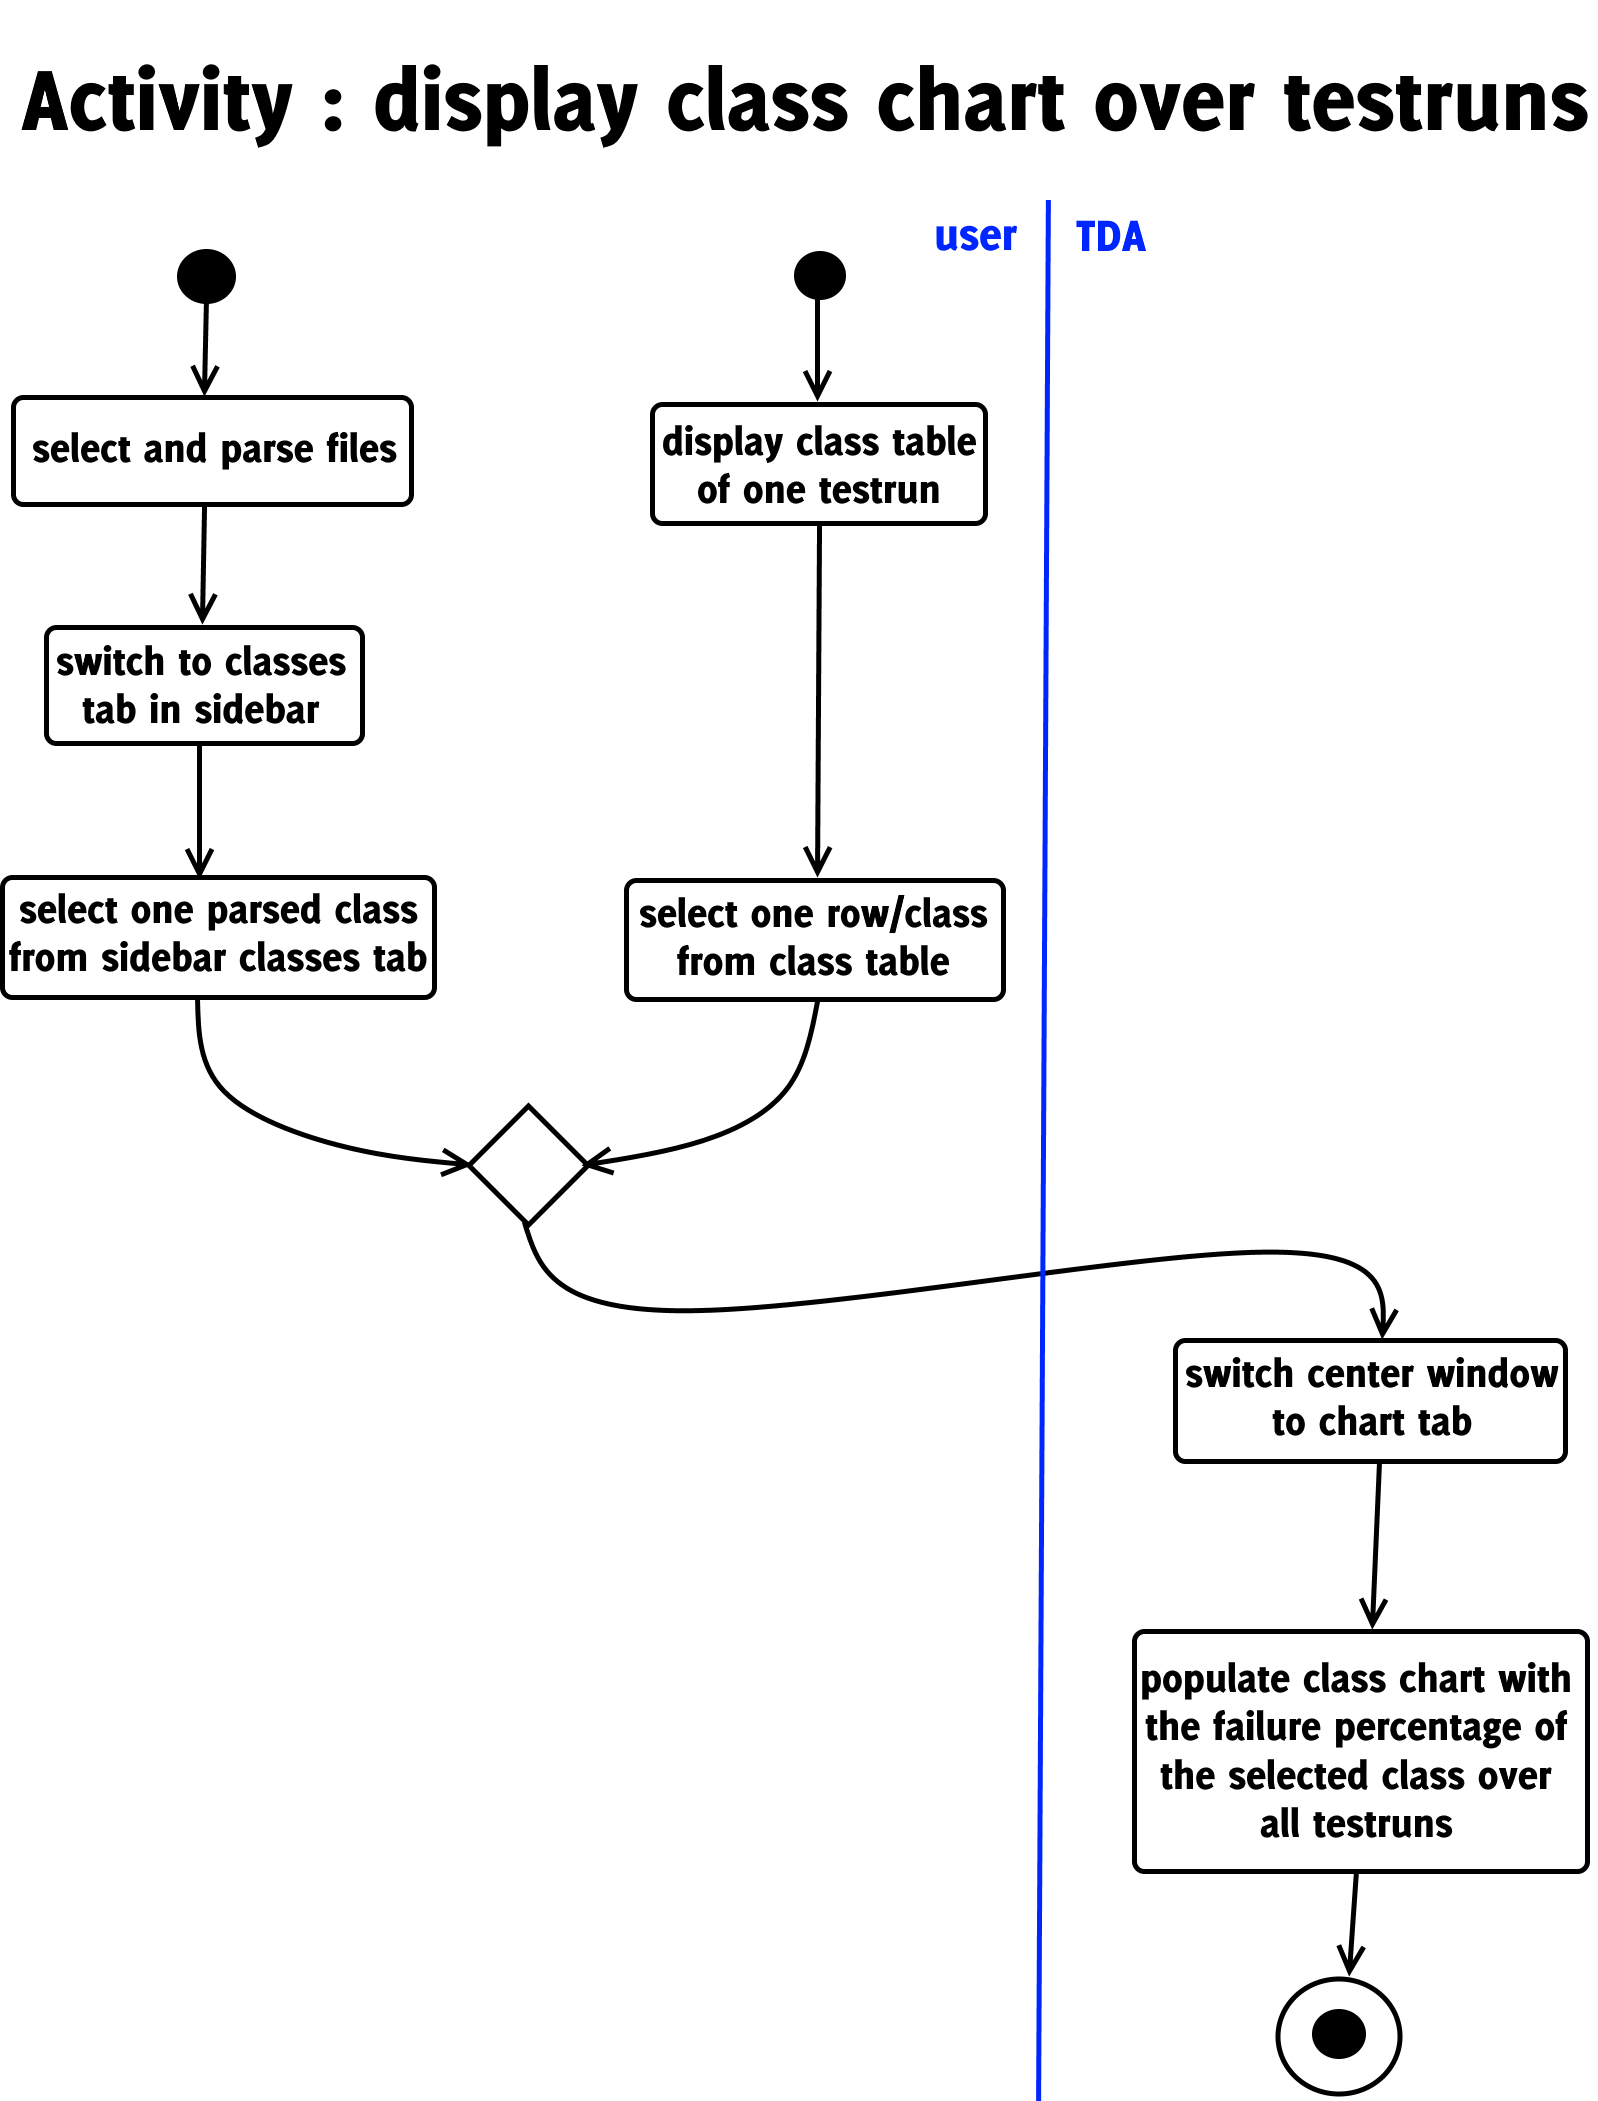
\includegraphics[scale=0.3]{pics/activityDisplayClassChartOverTestruns.png}
\caption{Activity Diagram: display class chart over testruns} 
\label{AD-DCCoTR}
\end{center}
\end{figure}
\ \\